
\documentclass{Setup/template_isec_class}

% Template ISEC/LaTeX, janeiro 2023
%--------------------------------------
\usepackage{Setup/template_isec_package}
%--------------------------------------

%--------------------------------------
% Obs#1
% Onde incluir todos os ficheiros (package)
% e instruções adicionais para este projeto
\usepackage{extras}
%--------------------------------------

\begin{document}

%--------------------------------------
% Obs#2
% Definir qual o título e quais os autores do trabalho
\newcommand{\titulotrabalho}{Sistema de Deteção e Prevenção de Intrusões}
\newcommand{\autorestrabalho}{Artur Falcão \& Gabriel Rodrigues \& Rodrigo Prazeres}
%--------------------------------------

\pagestyle{empty}

% Capa
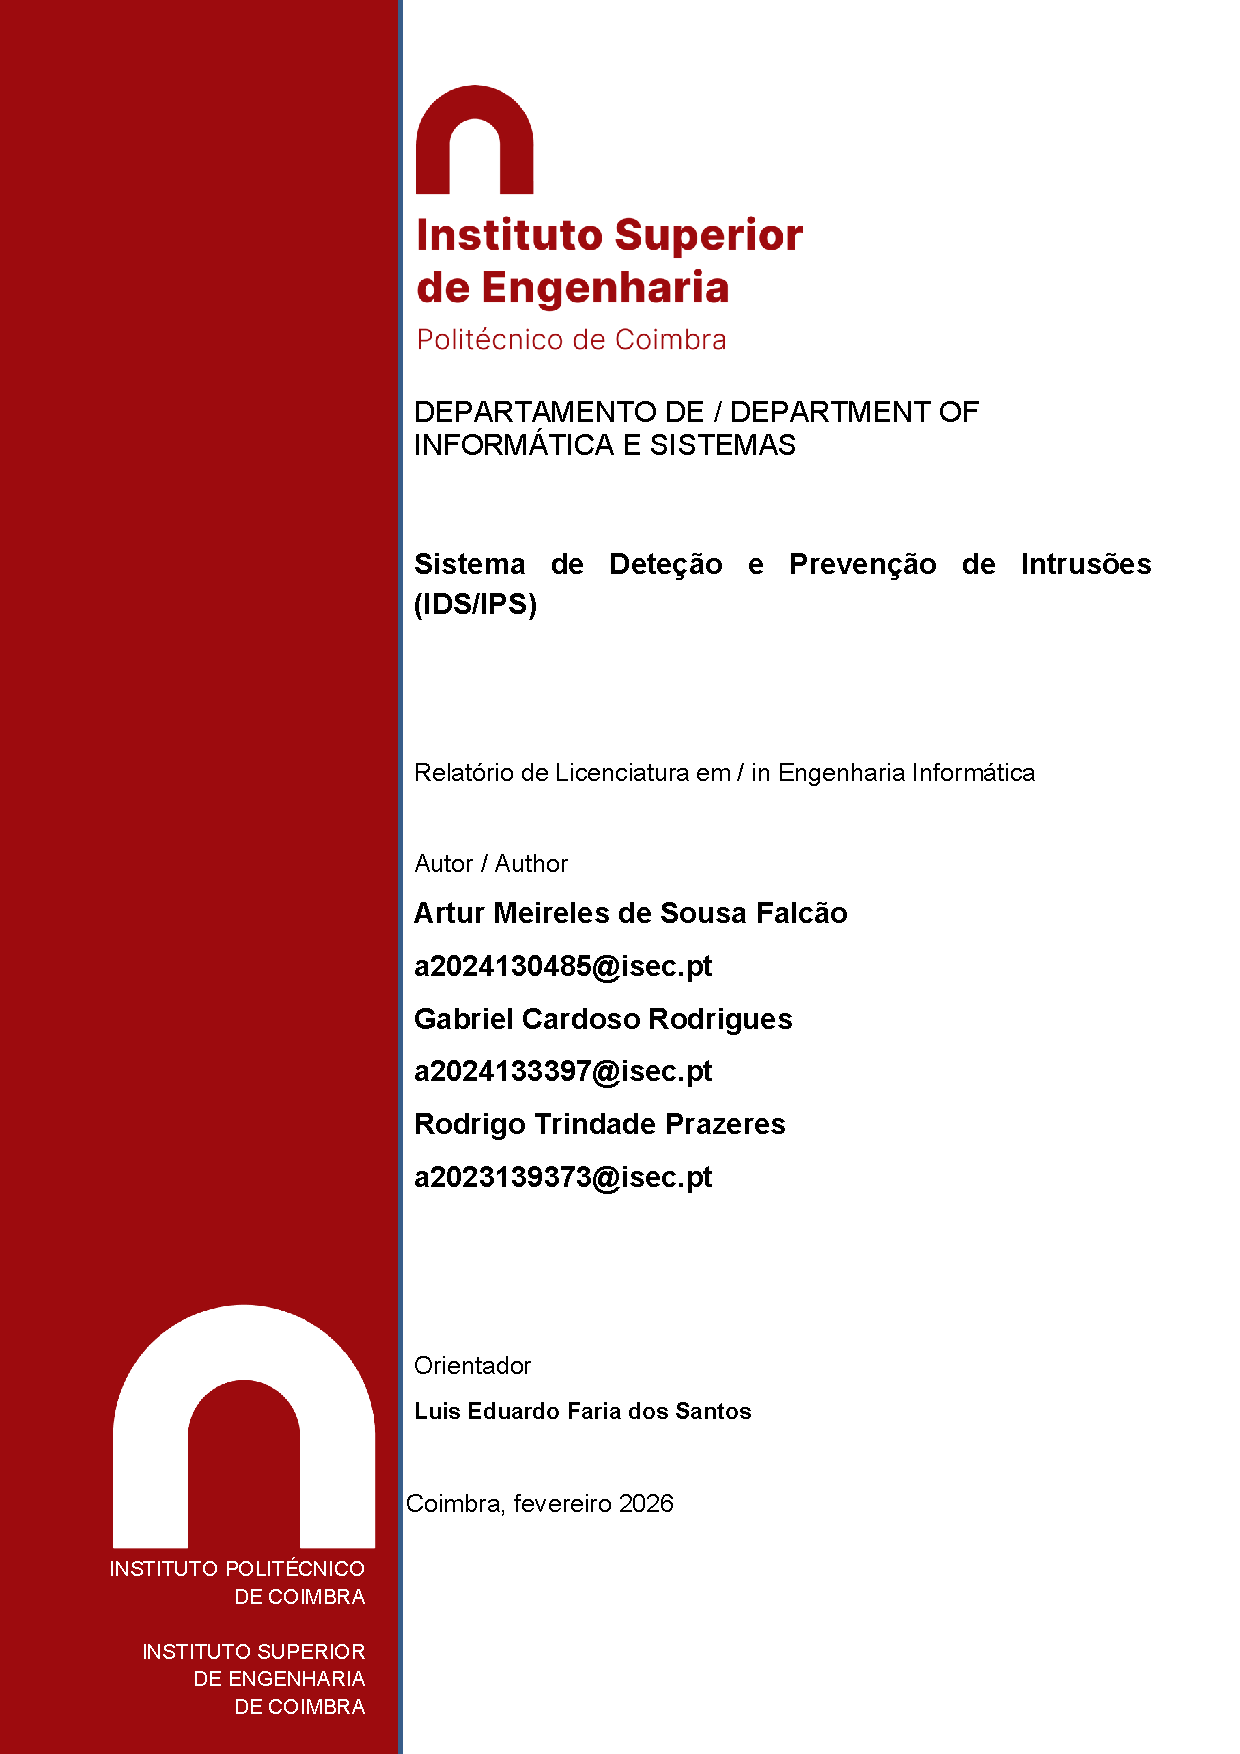
\includepdf{Inicio/capa}

\newpage

%--------------------------------------
\pagestyle{fancy}
\fancyhf{}
\fancyhead{}
\fancyhead[CO]{\nouppercase{\truncate{\headwidth}{\titulotrabalho}}}
\fancyhead[CE]{\nouppercase{\autorestrabalho}}
\renewcommand{\headrulewidth}{0pt}
\fancyfoot{}
\fancyfoot[CO,CE]{\thepage}
\setlength{\headheight}{14.5pt}
\fancypagestyle{plain}{}
%--------------------------------------

\pagenumbering{roman}

\renewcommand{\contentsname}{\'{I}ndice}

\phantomsection
\addcontentsline{toc}{chapter}{\'{I}ndice}
\tableofcontents

\newpage
\pagenumbering{arabic}

% Capítulo inicial
% Introdução

% Introdução
%--------------------------------------
\chapter{Introdução}
A segurança das infraestruturas de rede assume um papel cada vez mais relevante no contexto atual, caracterizado por um aumento significativo na sofisticação e frequência das ameaças informáticas. A monitorização contínua do tráfego de rede tornou-se um elemento essencial para a deteção precoce de comportamentos anómalos ou maliciosos e para a mitigação de incidentes de segurança, contribuindo para a preservação da confidencialidade, integridade e disponibilidade da informação.

Os \textbf{Sistemas de Deteção de Intrusões (IDS)} e os \textbf{Sistemas de Prevenção de Intrusões (IPS)} surgem como mecanismos fundamentais neste domínio. Um \textbf{IDS} opera de forma passiva, através da análise do tráfego de rede, com base na comparação com padrões previamente definidos ou na identificação de comportamentos anómalos. Sempre que deteta indícios de atividade maliciosa, emite alertas que permitem a adoção de medidas corretivas adequadas. Um \textbf{IPS}, por sua vez, introduz uma vertente ativa no processo de proteção e não se limita à deteção de ameaças, ou seja, procede ao bloqueio, à rejeição ou à mitigação de comunicações maliciosas em tempo real, de modo a salvaguardar a integridade, a confidencialidade e a disponibilidade dos sistemas.

Deste modo, estas soluções integram-se numa estratégia de defesa, na qual assumem funções de monitorização e controlo que complementam outras medidas de segurança, como \textit{firewalls} e políticas de controlo de acesso. Assim, no âmbito da Unidade Curricular de Segurança, revela-se fundamental a compreensão do seu funcionamento nas vertentes teórica e prática.


% Capítulo 2

% Segundo capítulo deste trabalho.
%--------------------------------------
\chapter{Proposta}

O presente projeto tem como objetivo o estudo teórico e a análise experimental de um \textbf{Sistema de Deteção de Intrusões (IDS)} e de um \textbf{Sistema de Prevenção de Intrusões (IPS)}. Estas ferramentas assumem um papel de particular relevância na segurança ativa de infraestruturas, através da análise do tráfego de rede com o intuito de identificar padrões associados a ataques conhecidos ou comportamentos anómalos. Conforme referido, um \textbf{IDS} caracteriza-se por um modo de operação passivo, com capacidade de identificar eventos potencialmente maliciosos e emitir alertas para posterior análise. Em contraste, um \textbf{IPS} incorpora mecanismos de resposta automática, que permitem a interrupção, filtragem ou mitigação de tráfego classificado como malicioso, com vista à preservação da integridade, confidencialidade e disponibilidade dos sistemas.

Entre as soluções de código aberto disponíveis, o motor \textbf{Suricata} destaca-se pelo seu elevado desempenho e suporte a Inspeção Profunda de Pacotes (Deep Packet Inspection – DPI). Neste contexto, o trabalho propõe a conceção e implementação de um guião laboratorial destinado a avaliar, de forma experimental, o funcionamento do Suricata em modo IDS e em modo IPS, bem como a sua eficácia na monitorização, deteção e eventual prevenção de ameaças \cite{suricata}.

\textbf{Prevê-se a utilização de}:

\begin{itemize}
    \item Plataforma de simulação de redes (GNS3);
    \item Máquina virtual com sistema operativo Linux;
    \item Motor Suricata configurado com conjuntos de regras comunitárias;
    \item Analisador de tráfego de rede (Wireshark) para captura e validação do tráfego analisado pelo IDS;
    \item Ferramentas de monitorização de desempenho e visualização de alertas.
\end{itemize}



\newpage

% Referências bibliográficas
\phantomsection
\addcontentsline{toc}{chapter}{Refer\^{e}ncias bibliogr\'{a}ficas}
\renewcommand{\bibname}{Refer\^{e}ncias bibliogr\'{a}ficas}

%-------------------
% Obs#3
% Descomentar uma das seguintes linhas, em alternativa, 
% consoante o estilo pretendido para as referências bibliográficas
\bibliographystyle{IEEEtran} % formatação segundo IEEE 
%\bibliographystyle{apacite} % formatação segundo APA 
%-------------------
\bibliography{bibliografia}

\newpage

\thispagestyle{empty}

% Última página
\input{Setup/ultima_pagina}

\end{document}

